%!TEX root = ../main.tex


%%%%%%%%%%%%%%%%%%%%%%%%%%%%%%%%%%%%%%%%%%%%%%%%%%%%%%%%%%%%%%%%%%%%%%%%%%%%%%%
%%%%%%%%%%%%%%%%%%%%%%%%%%%%%%%%%%%%%%%%%%%%%%%%%%%%%%%%%%%%%%%%%%%%%%%%%%%%%%%
\section{Introduction}
\label{sec:introduction}
%%%%%%%%%%%%%%%%%%%%%%%%%%%%%%%%%%%%%%%%%%%%%%%%%%%%%%%%%%%%%%%%%%%%%%%%%%%%%%%
%%%%%%%%%%%%%%%%%%%%%%%%%%%%%%%%%%%%%%%%%%%%%%%%%%%%%%%%%%%%%%%%%%%%%%%%%%%%%%%

Let us remind first the famous Pythagoras' theorem:

\begin{align}\label{eq:pythagore}
	\norm{x+y}^2 = \norm{x}^2 + \norm{y}^2 \enspace.
\end{align}

Note that \Cref{eq:pythagore} is ok only under some conditions.
In terms of visualisation, you can reference a figure easily using the command \Cref{fig:pythagore} or using Fig.~\ref{fig:pythagore}.

\begin{figure}[h!]
	\centering
	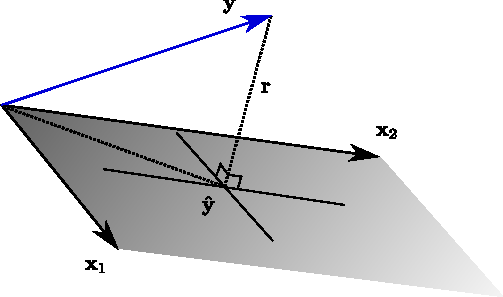
\includegraphics[width=0.8\textwidth]{residu_orth}
	\caption{Illustration of the residual orthogonality in least-squares.}
	\label{fig:pythagore}
\end{figure}


Also animage that is in the \texttt{prebuiltimages/} directory can also be loaded the same way:


\begin{figure}[h!]
	\centering
	
\includegraphics[width=0.2\textwidth]{umontpellier_logo}
	\caption{Illustration of a prebuiltimage available.}
	\label{fig:umontpellier_logo}
\end{figure}


Or subcaptions:

\begin{figure}
    \centering
    \begin{subfigure}[b]{0.43\textwidth}
    	\centering
        
\includegraphics[width=0.2\textwidth]{umontpellier_logo}%
        \caption{First example}
        \label{subfig:pythagore}
    \end{subfigure}
    \begin{subfigure}[b]{0.56\textwidth}
    	\centering
        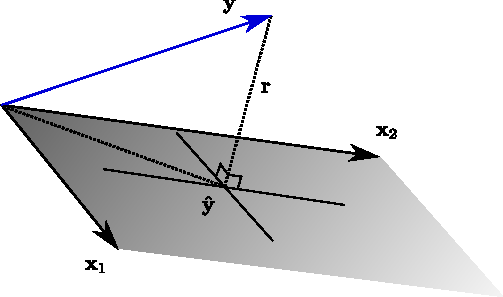
\includegraphics[width=0.5\textwidth]{residu_orth}%
        \caption{Second example}
        \label{subfig:logo}
    \end{subfigure}
    \caption{Exemples of side by side images}
    \label{fig:double_example}
\end{figure}


